\documentclass{tiba}
%\usepackage[figurename=Fig.]{caption}
%\usepackage{citation-style-language}
\begin{document}
\renewcommand{\figurename}{Fig.}
{
   % {
   %  \def\d{def}
   %  \edef\ed{edef}
   %  \gdef\gd{gdef}
   %  \xdef\xd{xdef}
   %  1 \d{}  \\
   %  2 \ed{} \\
   %  3 \gd{} \\
   %  4 \xd{} \\
}

% 1 \d \\
% 2 \ed \\
% 3 \gd \\
% 4 \xd \\

% 
% \def\a{a}
% \def\aa{a\a} % ou \edef ou \gdef ou \xdef
% \def\a{z}
% \aa


\newcommand*
{\ecrireLettre}[1]
{
\hspace{4ex}%
\ifthenelse{\equal{#1}{M}}{Cher Monsieur,}{Chère Madame,} 
J'ai le plaisir de vous inviter\dots
}

\ecrireLettre{M}


%\layout
%\lipsum[1-1]
%\newpage
%%%%%%%%%%%%%%%%%%%%%%%%%%%%%%%%%%%%%%%%%%%%%%%%%%%%%%%%%%%%%%%%%%%%%%%%%%%%%%%

%\thispagestyle{empty}
	\begin{center}
		\vfill
		
		%----------------- universite---------------
		\vfill
		\large{\textbf{
		\normalsize{\radp}      \\
		\normalsize{\ms}        \\
		%\normalsize{\dsp{\wil}}  \\
		\vfill
		\normalsize{\ispg}\\
		\normalsize{\ispr}\\
		}}
		\vfill
		%----------------------- image---------------------
		
\includegraphics[width=4cm,height=3.7cm]{img/msp.jpg}
		\vfill

		%------------------Numéro d'ordre---------------------
		%\begin{flushright}
			%Numéro d'ordre: ................
		%\end{flushright}
		
		%-----------------------Titre de votre projet-------------------------
		\fbox{
			\begin{minipage}{0.9\textwidth}
				\centering\large\textbf{Présentation}\\
				\centering\large\textbf{De la Monographie Sanitaire}\\
				\centering\large\textbf{De la Wilaya de MEDEA}\\
			\end{minipage}
		}
		\vfill
		
		%--------------------
		\large{présenté par:}\\
		\textbf{
		        \np \\
		        %...................\\
				    %...................\\
				    }
		\vfill
		%----------------------- image---------------------
		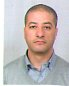
\includegraphics[width=4cm,height=3.7cm]{img/redha.jpg}
		\vfill
		%-----------------
		\underline{Sous la direction de:}\\
		\textbf {Dr R. CHOUTRI}
		\vfill
		%Soutenu le: jour mois année
	\end{center}

	\vfill

	% Devant le jury:
	% \bigskip
	 
	 %\begin{tabular}{ll}
	 %prof: ...................................................................\\
	 %prof: ...................................................................\\
	 %prof: ....................................................................\\

	 %\end{tabular}
	 %\vfill
		   
		 %\vfill
	 	 
	 \begin{center}
	 \emph{année: 2023}
	 \end{center}
	 
	%\vfill
	%\vfill
	%\vfill
	%\vfill
		\newpage

%%%%%%%%%%%%%%%%%%%%%%%%%%%%%%%%%%%%%%%%%%%%%%%%%%%%%%%%%%%%%%%%%%%%%%%%%%%%%%%

% \tableofcontents \newpage
% \listoftables    \newpage
% \listoffigures   \newpage

%%%%%%%%%%%%%%%%%%%%%%%%%%%%%%%%%%%%%%%%%%%%%%%%%%%%%%%%%%%%%%%%%%%%%%%%%%%%%%%

% %%%%%%%%%%%%%%%%%%%%%%%%%%%%%%%%%%%%%%%%%%%%%%%%%%%%%%%%%%%%%%%%%%%%%%%%%%%%%%%
\section{Infrastructures (Secteur Public)}
\subsection{Infrastructures}
\begin{table}[h!]
\begin{center}
\begin{tabular}{|p{6cm}|p{6cm}|p{1cm}|}
 \hline
 \multicolumn{2}{|l|}{Structures Sanitaires}                                    &Nbr\\
 \hline
 \multicolumn{2}{|l|}{Etablissements Publics Hospitaliers}                      &06 \\
 \multicolumn{2}{|l|}{Etablissements Publics de Santé de Proximité}             &07 \\
 \multicolumn{2}{|l|}{Polycliniques}                                            &00 \\
 \multicolumn{2}{|l|}{Salles de Soins}                                          &00 \\
 \multicolumn{2}{|l|}{UMC/UM (Hospitaliers)}                                    &00 \\
 \multicolumn{2}{|l|}{Points de  garde  (extrahospitaliers)}                    &00 \\
 \hline
 \multirow{3}{*}{Maternités}&Intégrées à une Polyclinique                       &00\\
                            &Intégrées  à une salle de soins                    &00\\
                            &Autonomes                                          &00\\ 
 \hline
 \multicolumn{2}{|l|}{UCTMR (unité de contrôle de la TBC et des maladies respiratoires)}                                                    &06 \\
 \multicolumn{2}{|l|}{MD (Maisons du diabétique (Centre de référence))}         &01 \\
 \multicolumn{2}{|l|}{CISM (centre  intermédiaire de santé mentale}             &00 \\
 \multicolumn{2}{|l|}{CISA (centre intermédiaire de soins  d’Addictologie)}     &01 \\
 \multicolumn{2}{|l|}{CDV (centre de depistage volentaire)}                     &01 \\
 \hline
 \multirow{2}{*}{UDS (unité de dépistage scolaire)}&Structures de la Santé      &00\\
                                                   &Structures de l’Education   &00\\
 \hline
 \multicolumn{2}{|l|}{CWS (Centre de transfusions sanguines wilaya)}            &01 \\
 \multicolumn{2}{|l|}{PTS (postes  de transfusions sanguines)}                  &05 \\
 
 \hline
 \multirow{2}{*}{Centres  d’hémodialyse publics}&Nombre de centres              &00\\
                                                &Nombre de générateurs          &00\\
 \hline
 \multicolumn{2}{|l|}{Centres Médico-Sociaux}                                   &00 \\
 \multicolumn{2}{|l|}{Centres de Médecine de Travail}                           &01 \\
 \hline
\end{tabular}
\end{center}
\caption{Infarstructures (Secteur Public)}
\label{table:1}
\end{table}
Table \ref{table:1} is an example of a referenced \LaTeX{} element.


%%%%%%%%%%%%%%%%%%%%%%%%%%%%%%%%%%%%%%%%%%%%%%%%%%%%%%%%%%%%%%%%%%%%%%%%%%%%%%%
\subsection{Les Structures Hospitalieres}
\begin{table}[h!]
\begin{center}
\begin{tabular}{|p{6cm}|p{1.5cm}|p{1.5cm}|p{1.5cm}|p{1cm}|}
 \hline
EPH                     &lits	    &Service	    &Sop	      &TDM \\
\hline
Médea	                  &538      &23           &12	        &02\\
Berouaghia	            &189	    &13	          &06	        &01\\
Ksarsar Elboukhari      &204	    &09	          &04	        &01\\
Ain boucif	            &111	    &09	          &02	        &00\\
Benislimane             &192	    &11	          &04	        &01\\
TablatT	                &120	    &09	          &03	        &01\\
Chellalet al adhaoura 	&60	      &04	          &01	        &00\\
\hline
TOTAL	                  &1414	    &78	          &32	        &06\\
\hline

\end{tabular}
\end{center}
\caption{Details des structures hospitalieres}
\label{table:2}
\end{table}
Table \ref{table:2} is an example of a referenced \LaTeX{} element.

\newpage
\subsection{Les Structures Extra-Hospitalieres}
\begin{table}[h!]
\begin{center}
\begin{tabular}{|p{5cm}|p{1cm}|p{1cm}|p{1cm}|p{1cm}|p{3cm}|}
\hline
\hline
\multirow{2}{*}{EPSP(EPSP)} &\multicolumn{3}{c|}{Polycliniques}&\multirow{2}{*}{SS} &\multirow{2}{*}{MAT} \\
                            \cline{2-4}
                            &H24 &H12  &TOT                     &                    &                     \\

%\multirow{2}{*}{EPSP}&\multicolumn{3}{|l|}{Polycliniques}& &\\ 
%\\
%                     &H24    &H12     &TOT    &SS    &MAT     \\
%\hline
\hline
Zoubiria	          &07	 &06	&13	 &34	&01 / 10 Lits\\
Berrouaghia	        &07	 &02	&09	 &33	&01 / 08 Lits\\
Ksar el boukhari	  &03	 &04	&07	 &17	&-           \\
Chahbounia	        &05	 &02	&07	 &21	&02 / 20 lits\\
CHELLALET ADHAOUERA	&05	 &09	&12	 &18	&01 / 13 Lits\\
BENISLIMANE	        &03	 &02	&07	 &29	&-           \\
TABLAT	            &05	 &04	&09	 &28	&-            \\
\hline
TOTAL	              &35	 &29	&64	 &180 &05 / 51 Lits\\
\hline

\end{tabular}
\end{center}
\caption{Details des structures Extra-Hospitalieres}
\label{table:3}
\end{table}
Table \ref{table:3} is an example of a referenced \LaTeX{} element.

\newpage
\section{Infrastructures (Secteur Privé)}
\begin{table}[h!]
\begin{center}
\begin{tabular}{|p{7cm}|p{1cm}|p{5cm}|}
\hline
Désignations                           & Nbr	          &Observations \\
\hline
Cliniques Médico-Chirurgicales(22 Lits)&01              &\\
Centres d’hémodialyse 	               &05	            &78 Générateurs\\
Laboratoires d’Analyses Médicales 	   &21	            &\\
Centres Imagerie Médicale (Radiologie) &09	            &dont 02 de Groupe\\
Cabinets Médicaux Spécialistes	       &236	            &dont 14 Cabinets de Groupe\\
Cabinets de Médecine Générale	         &179 	          &dont 09 Cabinets de Groupe\\
Cabinets de Chirurgie Dentaire	       &149 	          &dont 07 Cabinets de Groupe\\
Officines Pharmaceutiques 	           &203             &00\\
Agences ENDIMED	                       &21              &00\\
Cabinets de Sages-Femmes	             &05	            &00\\
Cabinets de Prothèse Dentaire	         &06              &00\\
Cabinets de Kinésithérapie	           &04              &00\\
Cabinets de Psychologues 	             &06              &00\\
Cabinets d’orthophonie	               &08              &00\\
Salles de Soins (Privées)	             &05              &00\\
Opticiens 	                           &17              &00\\
Unités de Transport Sanitaire	         &11	            &00\\
\hline
\end{tabular}
\end{center}
\caption{Infarstructures (Secteur Privé)}
\label{table:4}
\end{table}
Table \ref{table:4} is an example of a referenced \LaTeX{} element.



	
% % \newpage
\section{Principaux Ratios}
\begin{table}[h!]
\begin{center}
\begin{tabular}{|p{4cm}|p{1cm}|p{1cm}|p{1cm}|p{6cm}|}
\hline
\multirow{2}{*}{Désignations} &\multicolumn{3}{c|}{Polycliniques}&\multirow{2}{*}{Ratios}  \\
                              \cline{2-4}
                              &Public	&Privé &TOT                &                    \\
\hline
Lits (Hospitalisation )	                          &1558	&22	  &1580	&01 Lit/ 698 Hab.\\
Points de garde	                                  &35	  &-	  &35	  &01 PG/ 31 502 Hab.\\
Polycliniques	                                    &64	  &-	  &64	  &01 Poly/ 17 227 Hab.\\
Salles de soins	                                  &180  &05	  &185	&01 SS/ 5 960 Hab.\\
Médecins spécialistes	                            &431  &222	&653	&01 PS/ 1 688 Hab.\\
Médecins généralistes	                            &727  &188	&915	&01 MG/ 1 205 Hab.\\
Chirurgiens-dentistes	                            &144  &156	&300	&01 CH.D/ 3 675 Hab.\\
Pharmaciens	                                      &35	  &203	&238	&01 Pham/ 4 633 Hab.\\
Paramédicaux (ATS)	                              &3    &668	&54	  &3722	01 PM/ 296 Hab.\\
\hline
\end{tabular}
\end{center}
\caption{Principaux Ratios}
\label{table:44}
\end{table}
Table \ref{table:44} is an example of a referenced \LaTeX{} element.
	
% \newpage
\section{Moyens Humains}
\begin{table}[h!]
\begin{center}
\begin{tabular}{|p{6cm}|p{3cm}|p{3cm}|p{1cm}|}
\hline
Désignations des corps	       &Secteur Public	&Secteur Privé	&Total\\
\hline
Médecins Spécialistes	         &431	            &222	          &653\\
Médecins Généralistes	         &727	            &188	          &915\\
Chirurgiens-Dentistes	         &144	            &156	          &300\\
Pharmaciens	                   &35	            &203	          &238\\
Paramédicaux	                 &2478	          &34	            &2512\\
Aides-Soignants	               &1190	          &20	            &1210\\
Psychologues et Orthophonistes &132	            &14	            &146\\
Biologistes	                   &267	            &-	            &267\\
Personnel Administratifs	     &755	            &-	            &755\\
Autres Personnels	             &2000	          &-	            &2000\\
\hline
Total	                         &8159	          &837	          &8996\\
\hline
\end{tabular}
\end{center}
\caption{Moyens Humains}
\label{table:5}
\end{table}
Table \ref{table:5} is an example of a referenced \LaTeX{} element.
	
% \input{monographie/StructuresRéalisation.tex}	
% \input{monographie/PerformancesActivités.tex}	
% \newpage
\section{Principales Contraintes}

\begin{table}[h!]
\begin{center}
\begin{tabular}{|p{7cm}|p{7cm}|}
\hline
Contraintes	&Observations\\
\hline
&\\
\hline
\end{tabular}
\end{center}
\caption{Principales Contraintes}
\label{table:5555}
\end{table}
Table \ref{table:5555} is an example of a referenced \LaTeX{} element.
	

%%%%%%%%%%%%%%%%%%%%%%%%%%%%%%%%%%%%%%%%%%%%%%%%%%%%%%%%%%%%%%%%%%%%%%%%%%%%%%%

\includepdf[pages=14-15]{pdf_tuto/F20230_40_13.pdf}

%%%%%%%%%%%%%%%%%%%%%%%%%%%%%%%%%%%%%%%%%%%%%%%%%%%%%%%%%%%%%%%%%%%%%%%%%%%%%%%

\newpage
\begin{figure}[h]
\centering

\includegraphics[width=5cm, height=4cm]{img/msp.jpg}
\caption{Ministere de la santé}
\label{fig:mesh1}
\end{figure}

As you can see in the figure \ref{fig:mesh1}, the 
function grows near 0. Also, in the page \pageref{fig:mesh1} 
is the same example.


\begin{figure}[h]
\centering
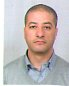
\includegraphics[width=5cm, height=4cm]{img/redha.jpg}
\caption{Dr Redha TIBA}
\label{fig:mesh2}
\end{figure}

%%%%%%%%%%%%%%%%%%%%%%%%%%%%%%%%%%%%%%%%%%%%%%%%%%%%%%%%%%%%%%%%%%%%%%%%%%%%%%%

% \index{a}aaa 
% \index{b}bbb
% \index{c}ccc\\

Ceci est un document avec une note de bas de page ici\footnote{voici la note}.

\newpage
\begin{tcolorbox}[colframe = orange, 
                  colback  = orange!50, 
                  boxrule  = 2pt, 
                  arc      = 6pt, 
                  title    = {Un titre}, 
                  coltitle = black] 
J'adore ce package ! \\ 
De toute mon âme ! 
\end{tcolorbox}

\begin{minipage}{0.45\linewidth} 
\begin{flushleft}  %left
\Large\textit{Auteur :} \\ Dr. Redha \textsc{TIBA} % Nom auteur 
\end{flushleft} 
\end{minipage} 
\hfill 
\begin{minipage}{0.45\linewidth} 
\begin{flushright} %right
\Large\textit{Superviseur :} \\ Dr. Reda \textsc{Choutri} 
\end{flushright} 
\end{minipage} 
%\textcolor{red}{tibaredha}
\newpage


% \LaTeX{} \cite{R-base} is a set of macros built atop \TeX{} \cite{drees}.

%%%%%%%%%%%%%%%%%%%%%%%%%%%%%%%%%%%%%%%%%%%%%%%%%%%%%%%%%%%%%%%%%%%%%%%%%%%%%%%

\cite{ref3}
%When using BiBTeX
\bibliographystyle{plain}% alpha  apalike  unsrt abbrv
\bibliography{bib/bib.bib}

%%%%%%%%%%%%%%%%%%%%%%%%%%%%%%%%%%%%%%%%%%%%%%%%%%%%%%%%%%%%%%%%%%%%%%%%%%%%%%%

%\newpage
%\printindex

\end{document}
